\begin{theo}
    \marginnote[0cm]{\cite{acamanes}}
    Pour tout entier naturel $n$ non nul, la \emph{somme de \textsc{Riemann}} associée à $f$ sur le segment $[a, b]$ est $S_n \defeq \frac{b-a}{n} \sum\limits_{k=0}^{n-1} f \left( a + k \frac{b-a}{n} \right)$. Si $f$ est continue par morceaux sur $[a, b]$, alors, 
    $$\lim_{n \to + \infty} S_n = \int_a^b f(t) \d t.$$
\end{theo}

\begin{marginfigure}[-3cm]
    %https://tex.stackexchange.com/questions/476702/riemann-sum-approaches-area-under-curve

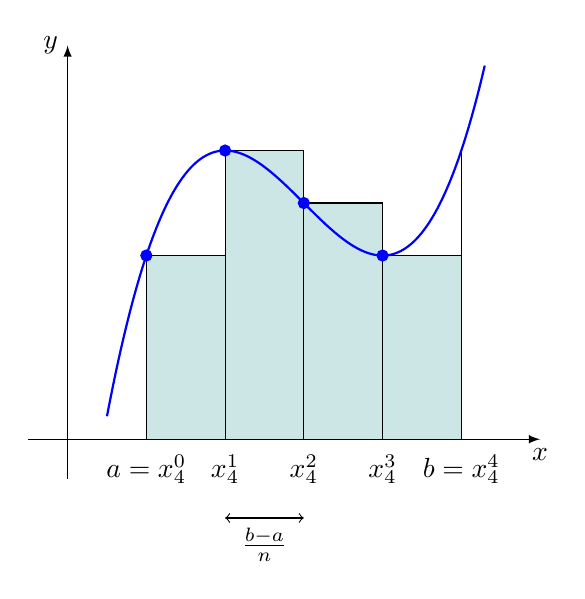
\begin{tikzpicture}[scale=1,declare function={f(\x)=((1/3)*(\x)^(3)-3*(\x)^(2)+8*\x-3;}]
\coordinate (start) at (.8,{f(.8)});
\coordinate (x0) at (1,{f(1)});
\coordinate (x1) at (2,{f(2)});
\coordinate (x2) at (3,{f(3)});
\coordinate (x3) at (4,{f(4)});
\coordinate (x4) at (5,{f(5)});
\coordinate (end) at (5.05,{f(5.05)});
\draw[fill=teal!20!white] (1,0) rectangle (2,{f(1)});
\draw[fill=teal!20!white] (2,0) rectangle (3,{f(2)});
\draw[fill=teal!20!white] (3,0) rectangle (4,{f(3)});
\draw[fill=teal!20!white] (4,0) rectangle (5,{f(4)});
\draw (5,0)--(5,{f(5)});
\draw [-latex] (-0.5,0) -- (6,0) node (xaxis) [below] {$x$};
\draw [-latex] (0,-0.5) -- (0,5) node [left] {$y$};
\foreach \x/\xtext in {1/a=x^0_{4} ,2/x^1_{4}, 3/x^2_{4} , 4/x^3_{4} , 5/b=x^4_{4}}
 \draw[xshift=\x cm] (0pt,3pt) -- (0pt,0pt) 
node[below=2pt,fill=white,font=\normalsize]
  {$\xtext$};
\draw[domain=.5:5.3,samples=200,variable=\x,blue,thick] plot ({\x},{f(\x)});                 
\foreach \n in {0,1,2,3}
\draw[blue,fill=blue] (x\n) circle (2pt) node[font=\normalsize] {$ $};    
\draw[<->] (2,-1)--(3,-1) node[below,midway] {$\frac{b-a}{n}$};      
\end{tikzpicture}
    \textcolor{red}{midway}
\end{marginfigure}

